\section{Background and Motivation}
Nuclear physics sheds light on the extremes. From the structure and reactions of atomic nuclei and hypernuclei to the formation and structure of some of the largest objects in the universe, neutron stars. One of the largest obstacles to these regimes comes from our incomplete knowledge of the nuclear interaction. Once a possible interaction is selected, the next obstacle is to solve for properties of many-body nuclear systems using the selected, and often complicated, interaction. Currently the popular choices for 2- and 3-body nuclear interactions come in two flavors, purely phenomenological and those based in Chiral Effective Field Theory ($\chi$EFT). There are a large number of methods that have been developed to solve various aspects of the many-body nuclear problem, and I will be using the Auxiliary Field Diffusion Monte Carlo (AFDMC) method to calculate ground state and low energy excitations as well as expectation values of quantities in these states. One of the early methods used in nuclear physics for this type of problem is the Hartree-Fock (HF) method. The HF method has been used to study condensed matter systems for most of a century \cite{hartree1928, fock1930, slater1951}, but wasn't used in nuclear physics until much later when the understanding of the nuclear interaction was improved \cite{zofka1970, gogny1986}. Before that simpler models were used such as the shell model and those models which were used to develope to shell model \cite{mayer1950_1,mayer1950_2}. HF begins with the mean field approximation which accounts for all inter-particle interactions by some average interaction. The wave function is usually assumed to be a Slater determinant, which is varied to minimize the energy. These calculations are often the starting place for other more sophisticated calculations. Such is the case with AFDMC and other Quantum Monte Carlo (QMC) methods.

Other notable methods are the basis set methods such as no core shell model \cite{navratil2009,barrett2013}, the coupled-cluster method \cite{hagen2014}, and the self-consistent Green's function method \cite{dickhoff2004,soma2014}. For these methods the wave function of the nuclear system is written in terms of a truncated basis, often a harmonic oscillator basis. The momentum cutoff of the basis needs to be higher than the important momenta of the interaction that is being used, in order to do calculations in momentum space. This means however that calculations with sharp potentials, like local hard core potentials, are difficult to do with basis set methods due to the relatively high momenta needed to describe such potentials. They do employ techniques such as Similarity Renormalization Group \cite{hergert2016} to soften these types of interaction, which consists of applying a regulator that will smoothly cut off the high momentum dependence of hard interactions such as the local contact interaction. This allows them to decrease the number of basis functions needed to describe the system accurately. One of the advantages of basis set methods is that they can use local and non-local, i.e. velocity dependent, potentials. Quantum Monte Carlo (QMC) methods, which I am using in this work, complement these basis set methods. QMC methods are currently limited to mostly local potentials\footnote{Currently, interactions that are linear in the momentum can be used. Higher order terms are treated perturbatively.} \cite{lynn2012}, but can converge for a wide variety of local Hamiltonians. Also, QMC methods do not inherently have the momentum cutoff limits or the poor scaling with basis set size of the basis set methods.

One of the most accurate QMC methods is the Green's Function Monte Carlo (GFMC) method, which has had good success calculating properties of light nuclei and nuclear matter using 2- and 3-body potentials as well as electroweak currents, elastic and inelastic form factors, and nuclear reactions \cite{carlson2015}. GFMC has been used to calculate binding energies as well as excitation spectra for nuclei up to $^{12}$C with good accuracy.
\begin{figure}[h!]
   \centering
   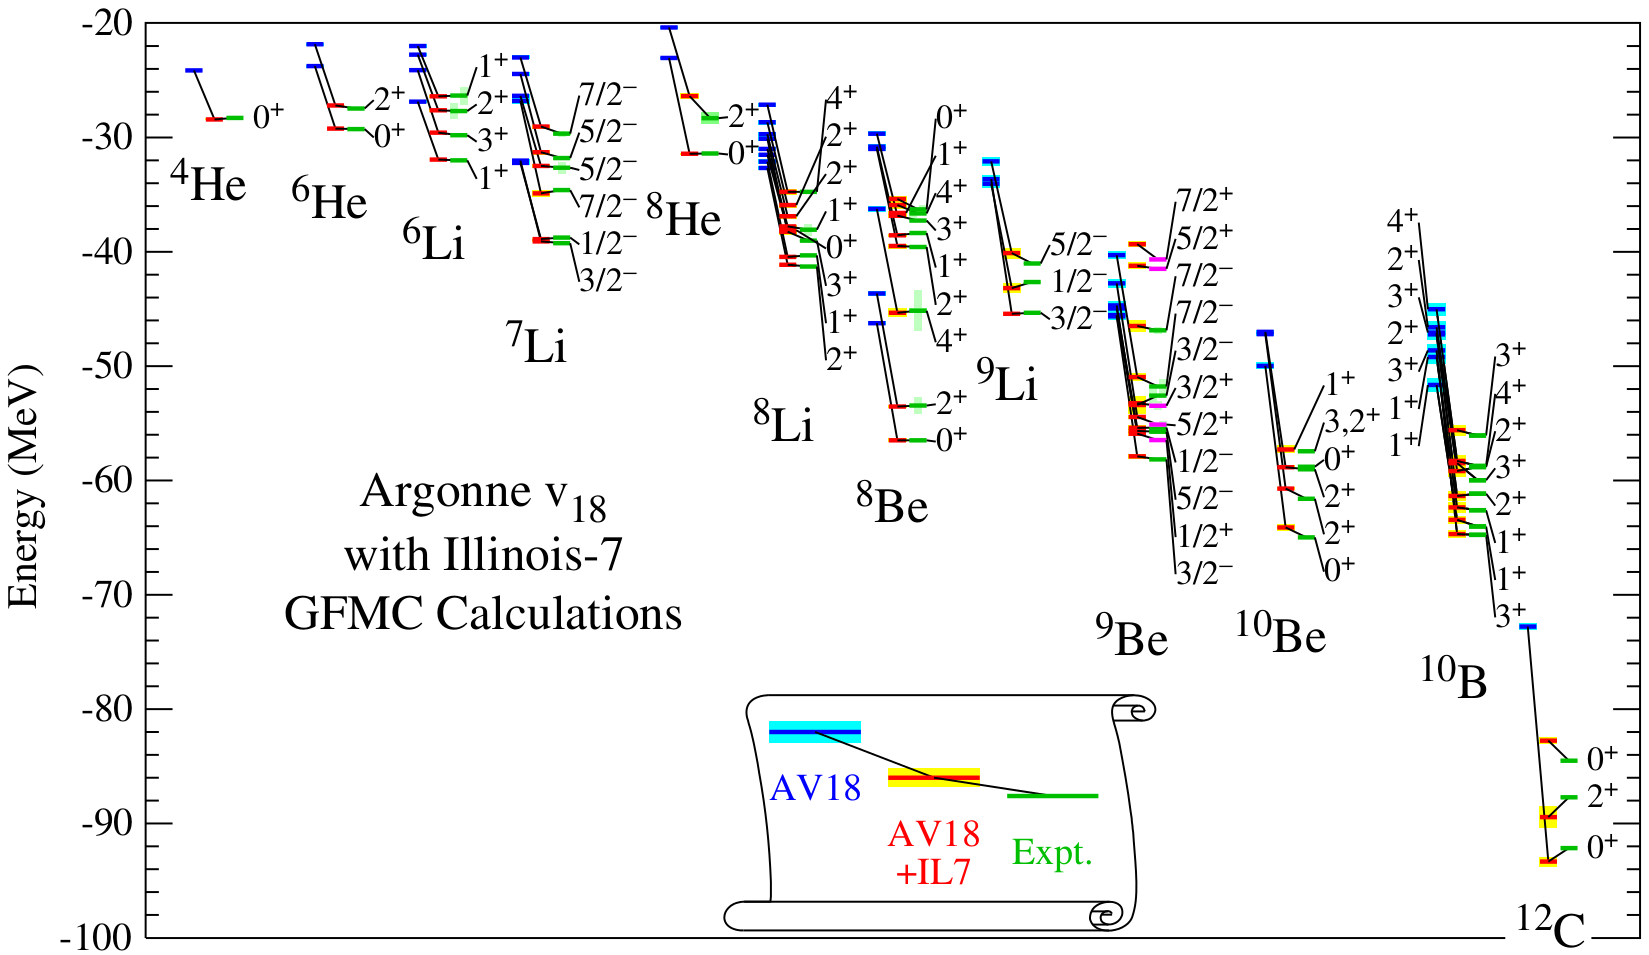
\includegraphics[width=0.8\textwidth]{figures/gfmc_energies.png}
   \caption{Ground and excited state energies calculated with GFMC calculated with the AV18 and AV18+IL7 potentials compared to experiment. Figure taken from \cite{carlson2015}.}
   \label{fig:energy_jaslin}
\end{figure}
Nuclear calculations using the GFMC method are limited due to the need to do explicit sums over spin-isospin states when calculating expectation values, which grows exponentially with the number of nucleons. The number of spin-isospin states for a system with $A$ nucleons and $Z$ protons is
\begin{equation}
   \frac{A!}{Z!(A-Z)!}2^A.
\end{equation}
\cite{schmidt1999} proposed the AFDMC method in 1999 which is practically identical to GFMC in its Monte Carlo sampling of spatial integrals, however AFDMC uses Monte Carlo to sample the spin-isospin sums as well. Since then AFDMC has been used to study light nuclei up to $^{40}$Ca \cite{gandolfi2007,lonardoni2017}, neutron stars \cite{gandolfi2014_2,gandolfi2012,tews2018}, the hyperon puzzle \cite{lonardoni2015,gandolfi2017_2}, as well as neutron and nuclear matter equation of states \cite{gandolfi2007_2,gandolfi2014,tews2018}, with both phenomenological interactions and interactions based on Chiral Effective Field Theory ($\chi$EFT) \cite{lonardoni2018_3,lonardoni2018} with 2- and 3- body forces. For recent reviews of QMC methods I refer the reader to \cite{carlson2015,lynn2019}.

Though this work has been used with the recently developed potentials based on $\chi$EFT and preliminary results are promising, we will primarily be using the AV6$'$ phenomenological potential for simplicity. The AV6$'$ potential is a refitting of the full Argonne $v18$ (AV18) \cite{wiringa1995} to only the first 6 operators, $(1,\si\cdot\sj,S_{ij})\otimes(1,\ti\cdot\tj)$, where the tensor term is $S_{ij} = 3\si\cdot\hat{r}_{ij}\sj\cdot\hat{r}_{ij}-\si\cdot\sj$. There has been much success with these phenomenological NN AV18 and 3N Urbana \cite{carlson1983} and Illinois potentials \cite{pieper2001}. However, phenomenological potentials have few connections to the underlying theory of QCD. Potentials based on $\chi$EFT have been developed in the past \cite{epelbaum2009}, but for some time they were only cast in momentum space or in a non-local form in position space, neither of which can be used with QMC. Recently the non-localities have been removed from the position space potentials up to next-to-next-to leading order (N2LO) in the chiral expansion and many AFDMC calculations have been done using these new potentials \cite{gezerlis2013}. These potentials have the same operator structure as the purely phenomenological potentials, but differ in the cuttoff choice and the order in which the various terms are included.

The goal of this study is to develop improved trial wave functions to be used with the AFDMC method. AFDMC was developed to extend the success of GFMC to larger systems. However, to calculate properties of larger systems accurately, better trial wave functions are needed. I will discuss the extension of these improved wave functions to some physical systems. The structure of this dissertation will be as follows.

In chapter 2, I will give an overview of the relevant QMC methods such as Variational Monte Carlo (VMC), Diffusion Monte Carlo (DMC), and AFDMC. I will also discuss the Hamiltonians used. Though I have only used purely phenomenological potentials in this work, an obvious extension to this work would be to apply these improved wave functions to the newly developed $\chi$EFT interactions, and so I will give a brief overview of those interactions as well.

In chapter 3, I will discuss the trial wave function. I will start by discussing the properties that we expect a good nuclear wave function to have and then I will introduce the most basic wave functions that satisfy these properties and are used as building blocks for many QMC and other calculations. I will then proceed to describe possible improvements to the existing wave functions and I will describe the specific improvements I have made as part of this work.

In chapter 4, I will extend the improved trial wave function to study the formation of alpha particles in neutron star crusts. I will show how important the improvements to the trial wave function are for describing correlated systems. In chapter 5 I will conclude and suggest possible extensions to the work that I have described.
